\documentclass[12pt]{article}

%%%%%%%%%%%%%%%%%%%%%%%%%%%%%%%%%%%%%%%%%%%%%%%%%%%%%%%%%%%%%%%%%%%%%%%%%%%%%%%%%%%%%%
\usepackage[numbers,sort]{natbib}
\usepackage{amsfonts, amsmath}
\usepackage{graphicx}
\usepackage{libertine}
\usepackage{fullpage}
\usepackage{booktabs}
\usepackage{float}
\usepackage[section]{placeins}
\usepackage{hyperref}
\usepackage{enumitem}
\hypersetup{
    colorlinks = true,
    linkcolor = blue,
    urlcolor  = blue,
    citecolor = blue,
    anchorcolor = blue}
\urlstyle{same}
%%%%%%%%%%%%%%%%%%%%%%%%%%%%%%%%%%%%%%%%%%%%%%%%%%%%%%%%%%%%%%%%%%%%%%%%%%%%%%%%%%%%%%

\begin{document}

\title{ST3247 SBI Final Report}
\date{}
\maketitle
\vspace{-2cm}

\noindent {\bf Github Repository:} \href{https://github.com/chongsun2002/st3247_project/tree/chongsun-changes}{chongsun2002/st3247\_project} (this goes to a branch. it is not a mistake)

\noindent {\bf Group Composition:}
\begin{enumerate}[nosep, leftmargin=10pt]
\item Tan Tag Han, A0214076L, taghan@u.nus.edu
\item Chua Chong Sun, A0273756R, chuachongsun@u.nus.edu
\end{enumerate}

\section{Introduction}

We consider an \emph{adaptive-network} SIR epidemic model in which a population of $N=200$ individuals is connected by a dynamic graph that co-evolves with the epidemic state. Each individual is in one of three states --- Susceptible (S), Infected (I), or Recovered (R) --- and the network is initialised as an Erd\H{o}s--R\'enyi graph $G(N, p_{\text{edge}}=0.05)$ with five randomly chosen seed infections. At every discrete time step $t = 1,\dots,T$ (with $T=200$), three phases are executed in sequence:

\begin{enumerate}[nosep, leftmargin=10pt]
    \item \textbf{Infection.} For every Susceptible--Infected (S--I) edge, the susceptible endpoint becomes infected with probability $\beta$. New infections are collected and applied synchronously.
    \item \textbf{Recovery.} Every infected node (including those infected in the current step) recovers with probability $\gamma$, transitioning permanently to the recovered (R) state.
    \item \textbf{Rewiring.} For every remaining S--I edge, with probability $\rho$ the susceptible endpoint cuts the edge and reconnects to a uniformly random non-neighbour, subject to a stale-edge check.
\end{enumerate}

The model has three unknown parameters: the infection rate $\beta$, the recovery rate $\gamma$, and the rewiring rate $\rho$. Our task is to infer their joint posterior distribution from $40$ observed replicates. Each replicate provides three pieces of information: the time series of the infected fraction, the time series of total rewiring events per step, and the empirical degree distribution at the final time step.

\paragraph{Why is the likelihood intractable?}
The state space of the model at each time step is the joint configuration of the SIR labels and the network topology. Even for moderate $N$, the number of possible (graph, labelling) configurations is astronomical, and the rewiring step in particular induces a non-Markovian dependence on \emph{which} edges still exist after the infection phase. As a result, the conditional density $p(y \mid \theta)$ of the observed trajectories cannot be written in closed form, nor evaluated in any practical way: even one-step transition probabilities require summing over an exponential number of possible new graph configurations. The model is, however, easy to \emph{simulate} forward in time. This is precisely the situation in which \emph{simulation-based inference} (SBI) is appropriate \citep{cranmer2020frontier}: rather than evaluating the likelihood, we use the simulator as a generative oracle and compare its output to the observed data through summary statistics. The remainder of this report develops, applies, and critically compares six SBI methods on this problem.

\section{Basic Rejection ABC}

\subsection{Algorithm}

Given a uniform prior $\pi(\theta)$ on $(\beta,\gamma,\rho)$, rejection ABC proceeds as follows \citep{pritchard1999population}: draw $\theta_i \sim \pi$, simulate $y_i \sim p(\cdot \mid \theta_i)$, compute summary statistics $S(y_i)$, and accept $\theta_i$ if the distance $d(S(y_i), S(y_{\text{obs}})) < \varepsilon$. The choice of summaries, distance, normalisation, and tolerance is critical.

\paragraph{Prior.} We use independent uniform priors:
\begin{equation*}
\beta \sim \mathcal{U}(0.05, 0.50), \quad \gamma \sim \mathcal{U}(0.02, 0.20), \quad \rho \sim \mathcal{U}(0.00, 0.80).
\end{equation*}
These ranges are wide enough to encompass plausible epidemic regimes (slow outbreaks to fast burnouts) without including extreme cases.

\paragraph{Summary statistics.} We use $d=12$ statistics grouped into three blocks:
\begin{itemize}[nosep, leftmargin=10pt]
    \item \emph{Infected time series} ($s_1$--$s_5$): peak infected fraction, time to peak (normalised by $T$), mean infected fraction (i.e.\ time-averaged area under the curve), epidemic duration (last time at which infected fraction $> 0.01$), and epidemic breadth (fraction of time steps with non-trivial infection).
    \item \emph{Rewiring time series} ($s_6$--$s_9$): total number of rewiring events, peak rewire count, time of peak rewire, and lag-1 autocorrelation of the rewire time series.
    \item \emph{Degree distribution} ($s_{10}$--$s_{12}$): mean of the final degree distribution, variance of the final degree distribution, and fraction of isolated nodes.
\end{itemize}
The observed summary vector $S(y_{\text{obs}})$ is computed by taking the per-replicate summary on each of the 40 observations and then taking the elementwise median. Using the median (rather than the mean) provides robustness against any pathological replicates.

\paragraph{Distance and normalisation.} The summaries live on very different scales (e.g.\ $s_6 \sim 500$ versus $s_1 \in [0,1]$). To make the Euclidean distance meaningful, each statistic is normalised by its median absolute deviation (MAD) computed over a pilot run of $2000$ prior simulations:
\begin{equation}
d(S, S') = \sqrt{\sum_{j=1}^{12} \left(\frac{S_j - S'_j}{\text{MAD}_j}\right)^2}.
\end{equation}
This is the same prescription used in standard ABC packages and has the advantage of being scale-free without requiring an externally-specified covariance.

\paragraph{Tolerance.} Rather than fixing $\varepsilon$ a priori, we use a quantile-based rule: we run $N_{\text{sim}}=50{,}000$ simulations and accept the smallest $1\%$ of distances. This ensures a fixed sample size (500 accepted) and lets us sweep over $q \in \{0.5\%, 1\%, 2\%, 5\%\}$ to study the bias--variance trade-off.

\subsection{Results}

Table~\ref{tab:rejection_quantile_sweep} reports the marginal posterior medians and 95\% credible intervals as the acceptance quantile $q$ varies. As expected, smaller $q$ produces tighter posteriors but more Monte Carlo noise from the smaller accepted sample. The $q=1\%$ choice strikes a reasonable balance.

\begin{table}[htb]
\centering
\small
\begin{tabular}{lcccccc}
\toprule
$q$ & $\hat\beta$ & $\hat\gamma$ & $\hat\rho$ & $\beta$ 95\% CI width & $\gamma$ 95\% CI width & $\rho$ 95\% CI width \\
\midrule
0.5\%  & 0.171 & 0.085 & 0.311 & 0.137 & 0.050 & 0.330 \\
1\%    & 0.172 & 0.086 & 0.302 & 0.147 & 0.055 & 0.390 \\
2\%    & 0.178 & 0.088 & 0.312 & 0.173 & 0.070 & 0.453 \\
5\%    & 0.189 & 0.093 & 0.329 & 0.205 & 0.086 & 0.536 \\
\bottomrule
\end{tabular}
\caption{Rejection ABC posterior medians and 95\% CI widths under different acceptance quantiles ($N_{\text{sim}}=50{,}000$, all 12 summaries).}
\label{tab:rejection_quantile_sweep}
\end{table}

\begin{figure}[htb]
\centering
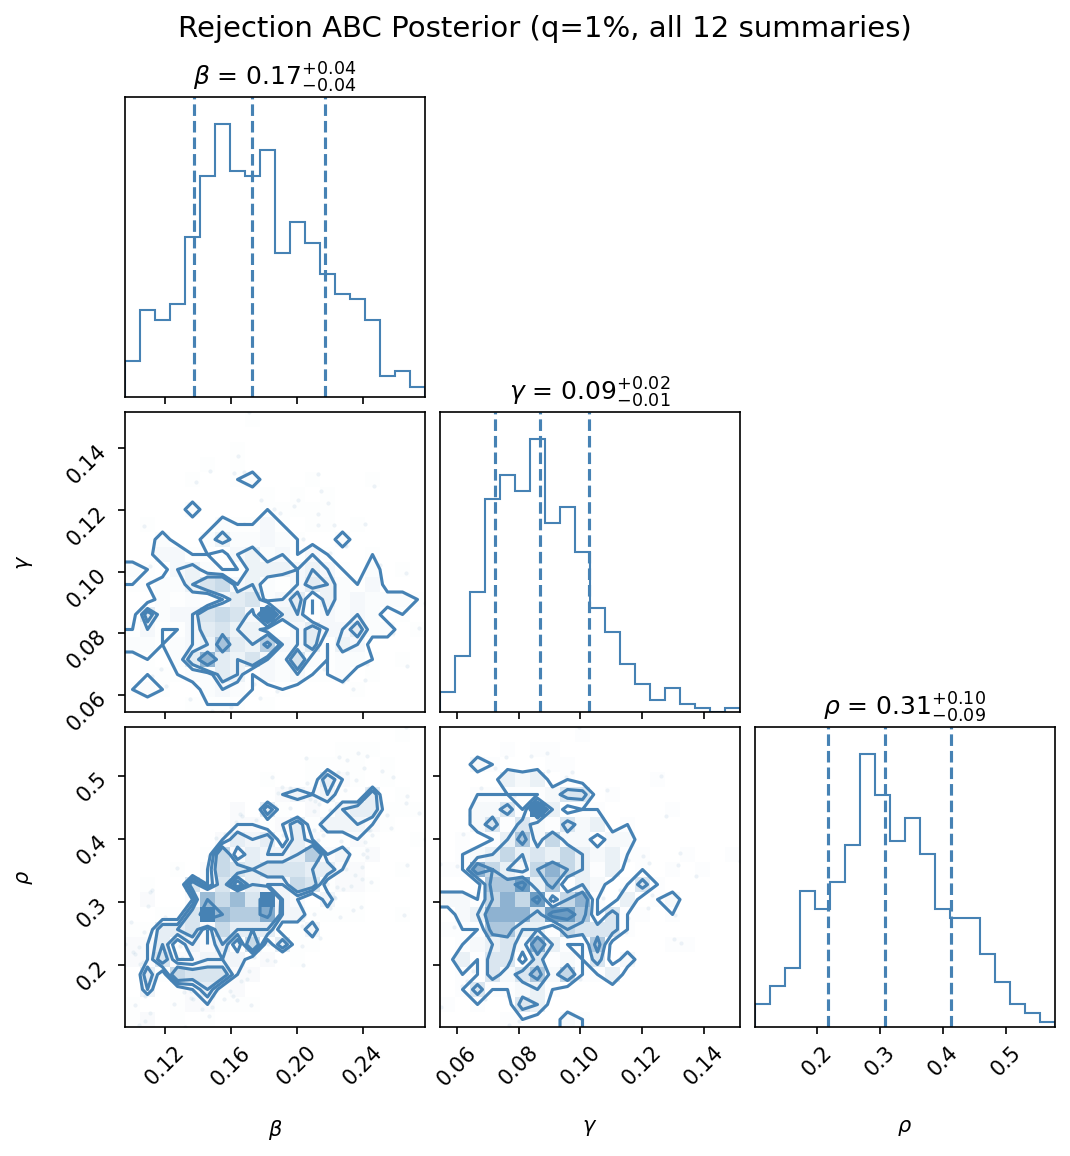
\includegraphics[width=0.75\textwidth]{../figures/rejection_abc_corner.png}
\caption{Approximate posterior over $(\beta,\gamma,\rho)$ from rejection ABC at $q=1\%$. Marginal histograms on the diagonal; pairwise scatter plots off-diagonal. The posterior is well-concentrated for $\beta$ and $\gamma$ but visibly broader for $\rho$, reflecting the harder identifiability of the rewiring rate.}
\label{fig:rejection_corner}
\end{figure}

The corner plot in Figure~\ref{fig:rejection_corner} shows the joint and marginal posteriors at $q=1\%$. The $\beta$ marginal is approximately Gaussian and concentrated near $0.17$, the $\gamma$ marginal near $0.086$, and the $\rho$ marginal near $0.30$. The posterior is widest in the $\rho$ direction, which we will explain in Section~\ref{sec:summaries}.

\paragraph{Posterior predictive check.} Figure~\ref{fig:posterior_predictive} overlays $200$ posterior predictive simulations (drawn from the NPE posterior; see Section~\ref{sec:advanced}) on the $40$ observed replicates for all three observable types. The predicted infected and rewiring trajectories bracket the observed replicates closely, and the predicted degree histogram matches the observed one within its 90\% envelope. This confirms that the inferred parameters produce data consistent with the observations.

\begin{figure}[htb]
\centering
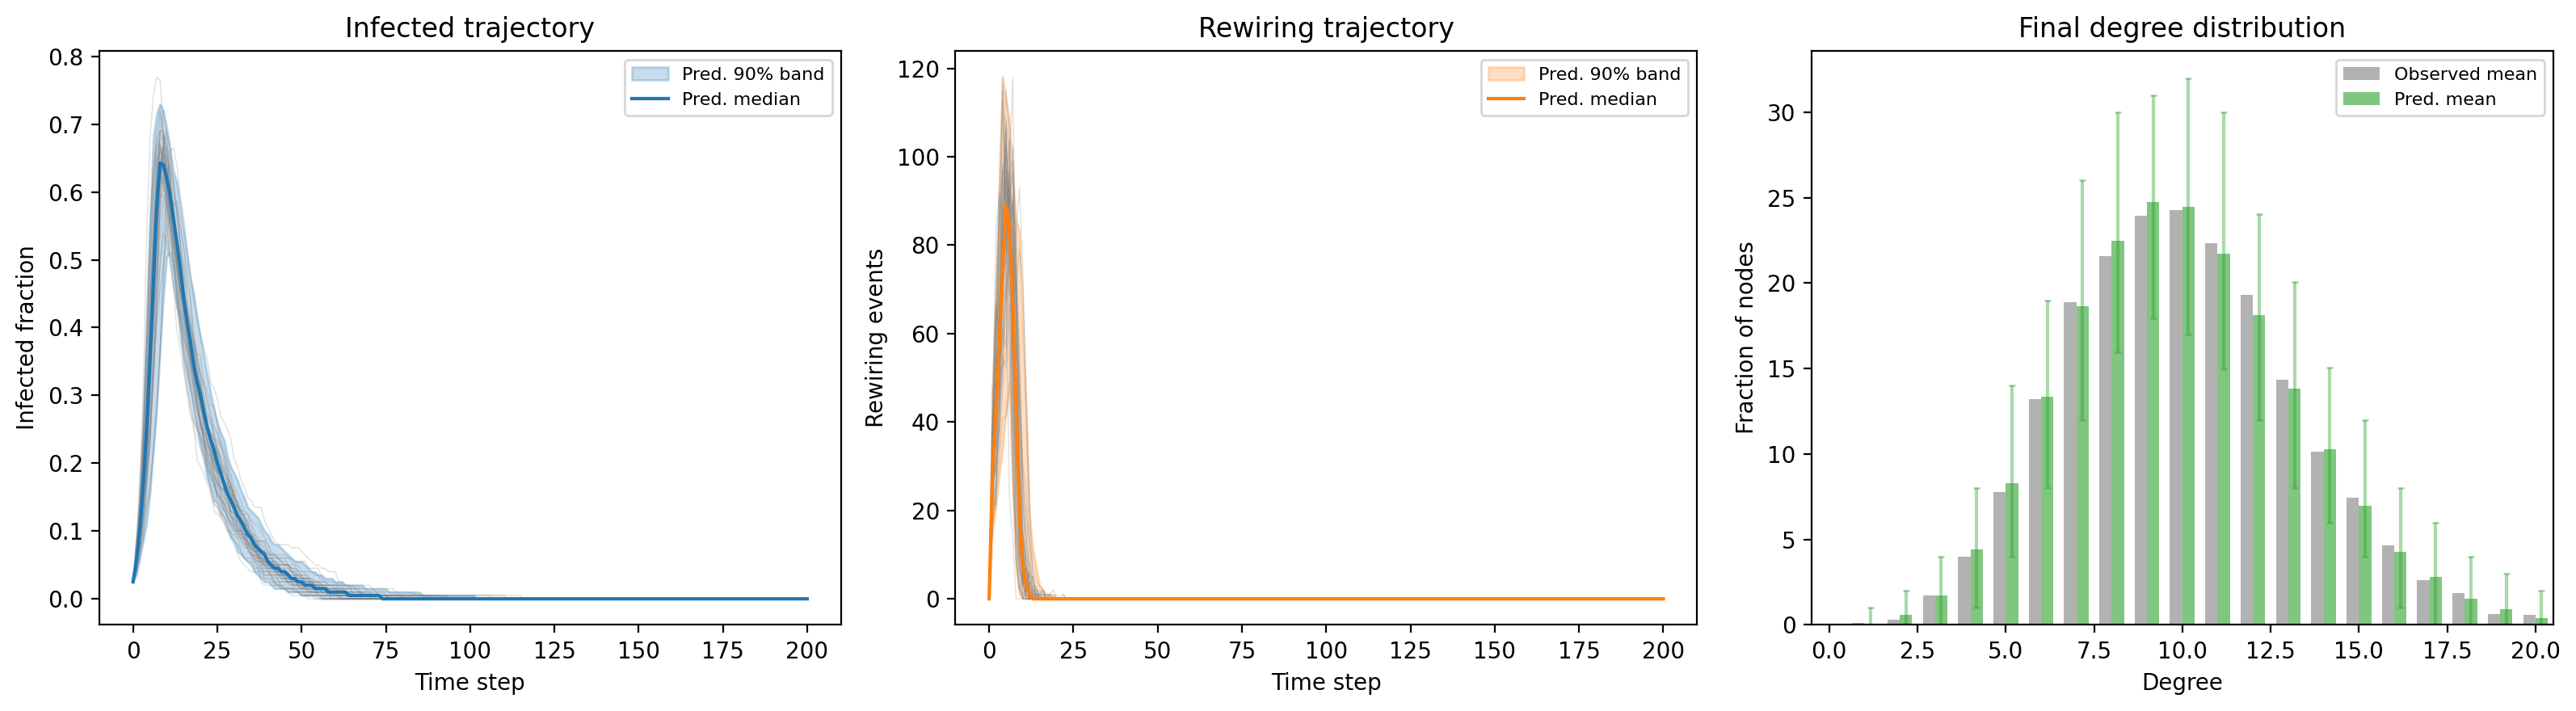
\includegraphics[width=0.95\textwidth]{../figures/posterior_predictive.png}
\caption{Posterior predictive check. Thin grey lines are the 40 observed replicates; the coloured band is the 5th--95th percentile of 200 simulations drawn from the NPE posterior, with the median shown as a solid line. Right panel: observed vs.\ predicted degree histograms with 90\% error bars.}
\label{fig:posterior_predictive}
\end{figure}

\paragraph{Quality of the estimates.} Rejection ABC gives a defensible first-order answer but has clear limitations. (i) The vast majority of simulations are wasted: $99\%$ of the parameter draws are discarded. (ii) The accepted region is determined entirely by the prior support and the distance threshold, with no adaptation to the geometry of the posterior. (iii) The posterior over $\rho$ remains noticeably wider than for the other parameters, suggesting either weak identifiability or that our distance is not informative enough about $\rho$. The next section addresses the second of these explanations.

\section{Summary Statistics Design}
\label{sec:summaries}

The choice of summary statistics is the single most consequential modelling decision in ABC. Information about a parameter is preserved only insofar as the summaries are sensitive to it; conversely, including uninformative statistics dilutes the distance and inflates the apparent posterior. We therefore investigate which summaries are informative for which parameters by running rejection ABC with six different summary subsets, all using the same $50{,}000$ simulations and acceptance quantile $q=1\%$.

\subsection{The $\beta$--$\rho$ confounding}

A key observation is that $\beta$ and $\rho$ have partially compensating effects on the epidemic curve. Higher $\beta$ accelerates spread along each S--I edge, but higher $\rho$ removes S--I edges from the network before they can transmit. From the standpoint of an observer who sees only the infected-fraction time series, a low-$\beta$/low-$\rho$ epidemic and a high-$\beta$/high-$\rho$ epidemic can produce very similar curves --- the slower spread of the former and the faster-but-truncated spread of the latter both yield comparable peak heights and durations. We therefore expect $\beta$ and $\rho$ to be strongly \emph{positively} correlated in the posterior when only infected statistics are used, and we expect rewiring or degree summaries (which directly observe the network dynamics) to weaken this confounding.

\subsection{Comparison of summary subsets}

Table~\ref{tab:summary_subsets} reports posterior 95\% CI widths and the Pearson correlation $\hat r(\beta,\rho)$ in the accepted samples for each of six subsets, all using the same $50{,}000$ simulations and acceptance quantile $q=1\%$.

\begin{table}[htb]
\centering
\small
\begin{tabular}{lccccc}
\toprule
Summary subset & $|\text{CI}_\beta|$ & $|\text{CI}_\gamma|$ & $|\text{CI}_\rho|$ & $\hat r(\beta,\rho)$ & $\hat r(\beta,\gamma)$ \\
\midrule
Infected only ($s_1$--$s_5$)        & 0.223 & \textbf{0.039} & 0.753 & $+0.886$ & $+0.044$ \\
Rewiring only ($s_6$--$s_9$)        & 0.181 & 0.167 & \textbf{0.278} & $+0.803$ & $+0.513$ \\
Degree only ($s_{10}$--$s_{12}$)    & 0.425 & 0.169 & 0.628 & $+0.350$ & $-0.028$ \\
Infected + Rewiring                 & \textbf{0.148} & 0.051 & 0.399 & $+0.725$ & $+0.123$ \\
Infected + Degree                   & 0.188 & 0.050 & 0.589 & $+0.772$ & $+0.089$ \\
All 12                              & 0.147 & 0.055 & 0.390 & $+0.714$ & $+0.133$ \\
\bottomrule
\end{tabular}
\caption{Posterior 95\% CI widths and pairwise correlations of the rejection ABC accepted samples under six summary subsets ($q=1\%$, $N_{\text{sim}}=50{,}000$). Bold marks the smallest value in each column.}
\label{tab:summary_subsets}
\end{table}

Several conclusions emerge, some confirming and some refining our mechanistic intuition:
\begin{itemize}[nosep, leftmargin=10pt]
\item \textbf{Infected-only summaries leave $\rho$ almost unconstrained.} Using only $s_1$--$s_5$, the $\rho$ CI width is $0.75$, nearly the full prior range $[0,0.8]$, and the $\beta$--$\rho$ correlation is $+0.886$ --- a near-degenerate ridge in $(\beta,\rho)$ space. Strikingly, however, the $\gamma$ CI is the \emph{narrowest} of any subset ($0.039$). This makes sense: $\gamma$ governs the speed at which the infected curve decays back to zero, and the infected time series is precisely where this decay is observed. Infected statistics are highly informative for $\gamma$ but extremely weak for $\rho$.
\item \textbf{Rewiring statistics are the single most informative source for $\rho$.} Using only $s_6$--$s_9$ shrinks the $\rho$ CI to $0.28$ --- the narrowest of any subset, including the full set of 12. The rewiring counts directly observe the rate at which edges are cut and reconnected, so they provide the most direct evidence of $\rho$. The $\beta$--$\rho$ correlation, however, remains high ($+0.80$); knowing $\rho$ alone is not enough to disentangle it from $\beta$ when the infection curve itself is hidden.
\item \textbf{Degree summaries are weak on their own.} The final-time degree histogram alone produces the widest CIs across the board: degree information is too coarse to recover dynamic parameters in isolation. Combined with infected statistics, however, it adds very little ($\rho$ CI shrinks only marginally from $0.75$ to $0.59$).
\item \textbf{Infected + Rewiring captures the bulk of the information.} The CI widths for this subset $(0.148, 0.051, 0.399)$ are essentially the same as for all 12 statistics $(0.147, 0.055, 0.390)$. Adding the degree statistics on top provides only marginal extra precision. Practically, the rewiring time series is the indispensable second source.
\item \textbf{The residual $\beta$--$\rho$ confounding is real, not a defect of our distance.} Even with all 12 statistics, $\hat r(\beta,\rho) = +0.71$. This is structural: $\beta$ and $\rho$ are partially \emph{exchangeable} in their effect on the observable summaries, and no choice of distance can fully separate them on this dataset. Any honest report of the posterior must respect this correlation.
\end{itemize}

\begin{figure}[htb]
\centering
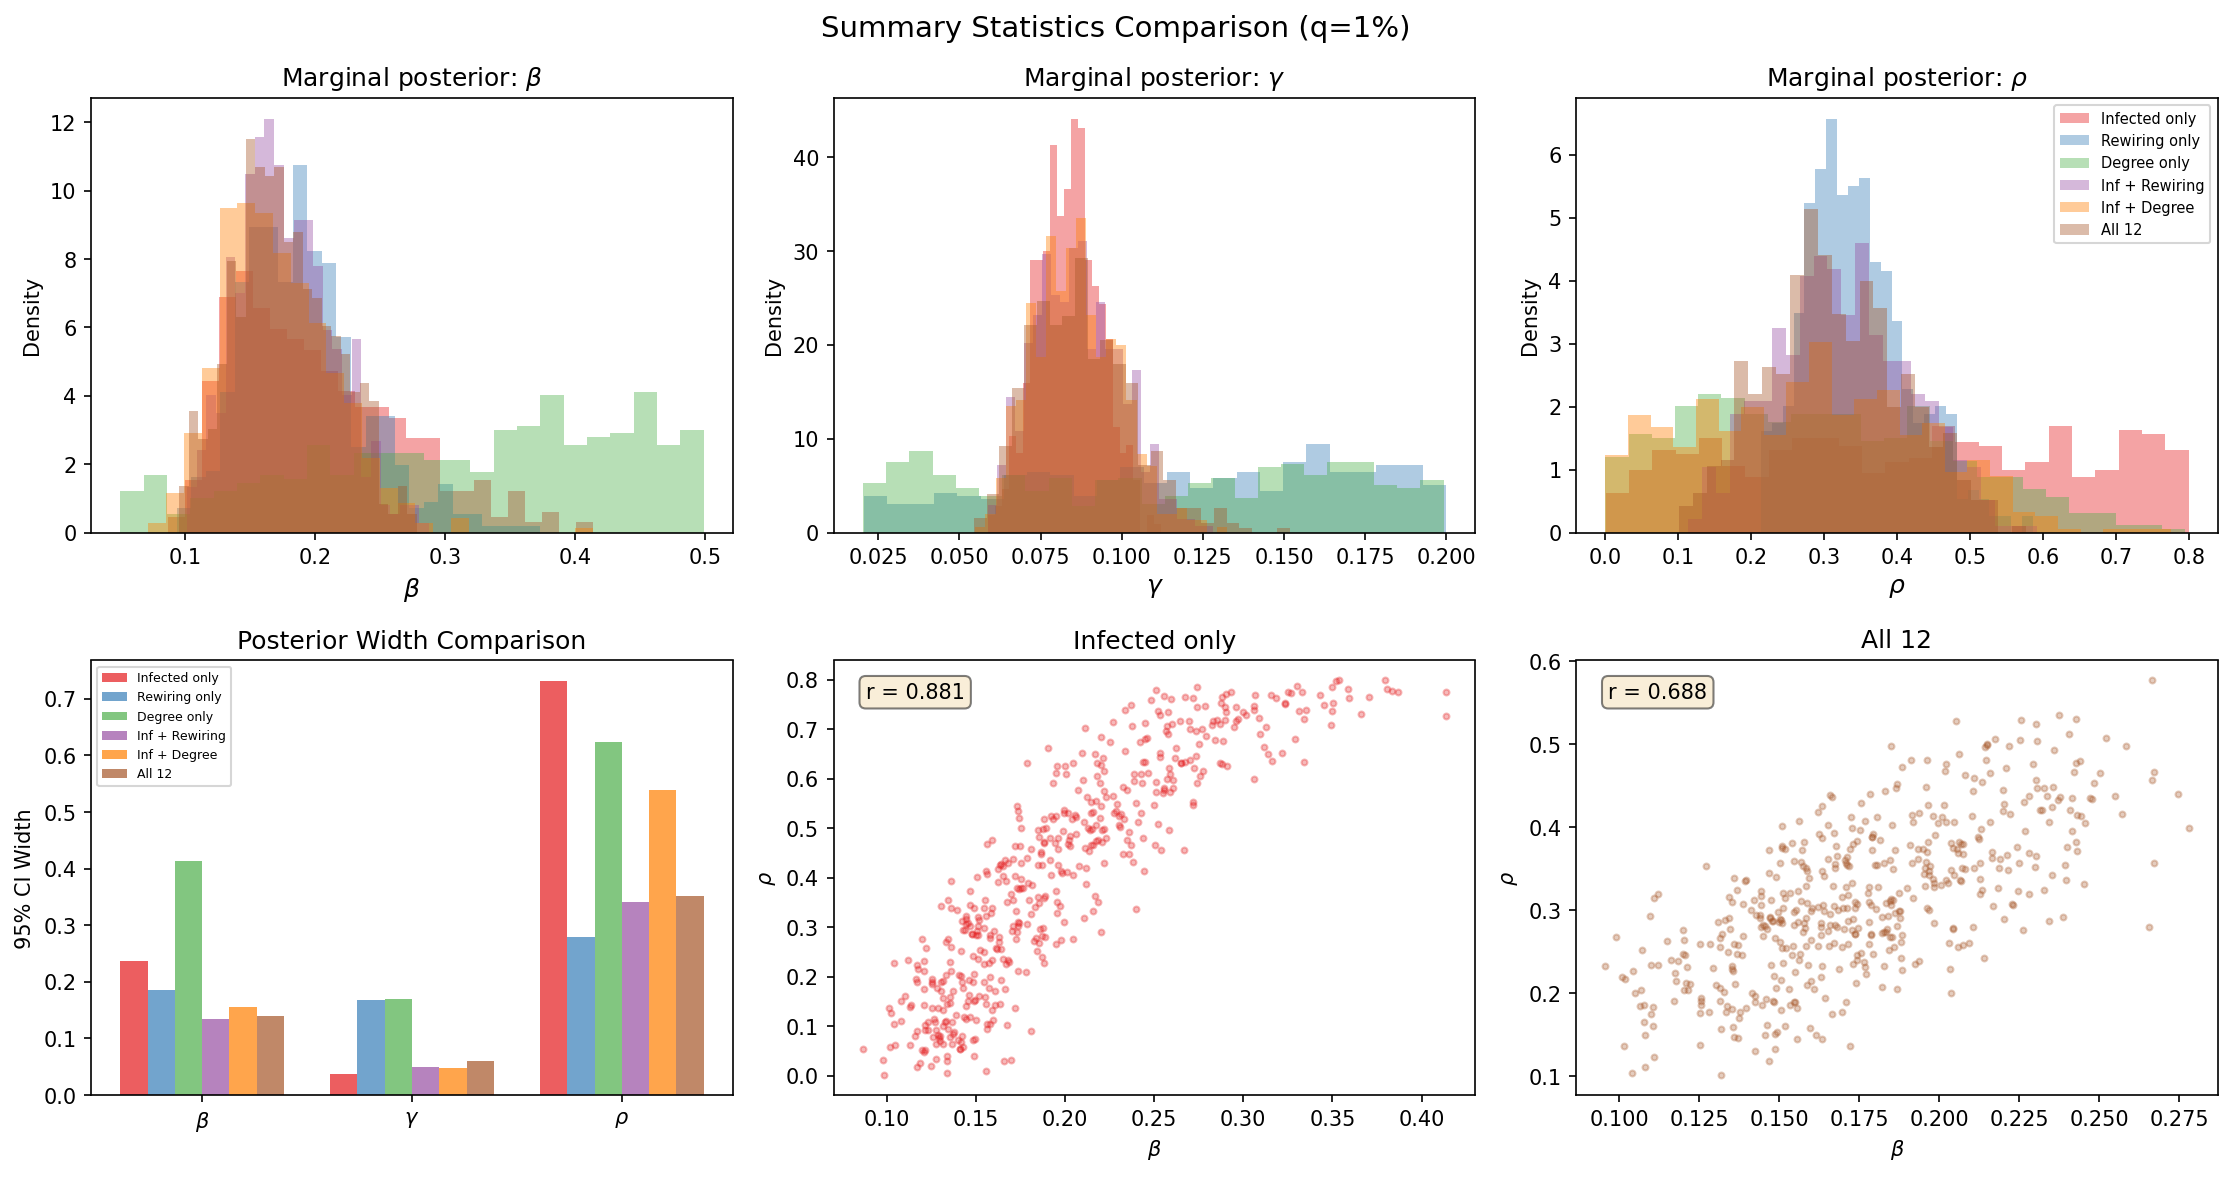
\includegraphics[width=0.80\textwidth]{../figures/summary_stats_comparison.png}
\caption{Posterior marginals (top row) and 95\% CI width comparison (bottom-left) for the six summary subsets, plus joint $(\beta,\rho)$ scatter plots for the infected-only and full-12 cases (bottom centre and right). The diagonal ridge is clearly visible when only infected statistics are used and is broken once rewiring or degree statistics are added.}
\label{fig:summary_subsets}
\end{figure}

\paragraph{Take-away.} The poor identifiability of $\rho$ in the basic rejection ABC results is not a defect of the inference procedure but a real feature of the model: $\rho$ is genuinely hard to pin down without observing edge dynamics directly. The rewiring counts almost perfectly addresses this. We therefore use all 12 summaries in the remainder of the report.

\section{Advanced Methods}
\label{sec:advanced}

We now compare five advanced SBI methods against the basic rejection ABC baseline. The first three (regression-adjusted ABC, ABC-MCMC, SMC-ABC) are classical ABC variants that aim to make better use of the simulation budget. The fourth (synthetic likelihood) replaces the ABC tolerance with an explicit Gaussian likelihood approximation. The fifth (Neural Posterior Estimation) uses a normalising flow to learn the posterior amortised over all observations.

\subsection{Regression-adjusted ABC}

Regression-adjusted ABC \citep{beaumont2002approximate} post-processes the rejection ABC accepted samples by fitting a local weighted linear regression of the parameters on the summaries, then shifting each accepted $\theta_i$ in the direction predicted to compensate for the residual gap $S_i - S_{\text{obs}}$:
\begin{equation}
\theta_i^* = \theta_i - \hat B^\top (S_i - S_{\text{obs}}),
\end{equation}
where $\hat B$ is the matrix of weighted least-squares coefficients and the weights are Epanechnikov kernel weights $w_i = 1 - (d_i / d_{\max})^2$. We use the larger acceptance quantile $q=5\%$ ($2{,}500$ samples) to give the regression more data to fit. This adjustment costs essentially nothing (it reuses the existing simulations and the regression solve takes $0.013$\,s) but typically tightens the posterior dramatically.

\subsection{ABC-MCMC}

ABC-MCMC \citep{marjoram2003markov} runs a Markov chain whose stationary distribution is the ABC posterior. In the general algorithm (Algorithm~F of \citeauthor{marjoram2003markov}), one proposes $\theta' \sim q(\cdot \mid \theta_{\text{cur}})$, simulates a dataset $y' \sim p(\cdot \mid \theta')$, and if the distance $d(S(y'), S_{\text{obs}}) < \varepsilon$, accepts $\theta'$ with Metropolis--Hastings probability $\min\bigl(1,\; \pi(\theta')\,q(\theta \mid \theta')\,/\,[\pi(\theta)\,q(\theta' \mid \theta)]\bigr)$; otherwise the chain stays at~$\theta$. In our setting the prior $\pi$ is uniform and the proposal $q$ is a symmetric Gaussian random walk, so both the prior ratio and the proposal ratio equal one whenever $\theta'$ lies in the prior support, and the acceptance criterion reduces to a hard tolerance check. For our implementation we initialise the chain at the median of the rejection ABC accepted set, take $\Sigma_q = 0.5 \cdot \widehat{\text{Cov}}(\theta_{\text{rej}})$, set $\varepsilon = 1.2 \times$ the rejection threshold, and run for $30{,}000$ iterations with $5{,}000$ burn-in. Effective sample sizes (ESS) are computed from the autocorrelation function.

\subsection{SMC-ABC}

Sequential Monte Carlo ABC \citep{sisson2007sequential, beaumont2009adaptive} maintains a population of weighted particles that is propagated through a sequence of decreasing tolerances $\varepsilon_0 > \varepsilon_1 > \dots$ The basic SMC-ABC framework was introduced by \citet{sisson2007sequential}; we follow the adaptive variant of \citet{beaumont2009adaptive}, which sets each new tolerance as a quantile of the current distances and uses a perturbation kernel whose covariance is $2\widehat{\text{Cov}}$ of the alive particles. At each generation, particles are resampled in proportion to their weights, perturbed by this Gaussian kernel, and accepted at the tighter tolerance. Importance weights are recomputed as
\begin{equation}
w_i^{(t)} \propto \frac{\pi(\theta_i^{(t)})}{\sum_j w_j^{(t-1)} K(\theta_i^{(t)} \mid \theta_j^{(t-1)})}.
\end{equation}
We use $1{,}000$ particles, $10$ generations, and an adaptive tolerance $\varepsilon_t = $ median of distances at generation $t-1$.

\subsection{Synthetic likelihood}

The synthetic likelihood method \citep{wood2010statistical} replaces the ABC distance with an explicit Gaussian likelihood: at each proposed $\theta$, simulate $N_r=200$ replicates, estimate the mean $\hat\mu_\theta$ and covariance $\hat\Sigma_\theta$ of the summary vector, and evaluate
\begin{equation}
\log L_S(\theta) = -\frac{1}{2}(S_{\text{obs}} - \hat\mu_\theta)^\top \hat\Sigma_\theta^{-1}(S_{\text{obs}} - \hat\mu_\theta) - \frac{1}{2}\log|\hat\Sigma_\theta|.
\end{equation}
This approximate likelihood is then explored by a Metropolis--Hastings random walk. We follow Wood's reference R implementation and use Campbell's robust covariance estimator with QR preconditioning, which down-weights extreme replicates and stabilises the matrix inversion. We run $5{,}000$ MCMC iterations with $1{,}000$ burn-in, for a total of $10^6$ simulator calls.

\subsection{Neural Posterior Estimation}

Neural Posterior Estimation (NPE) \citep{papamakarios2016fast, greenberg2019automatic} trains a conditional density estimator $q_\phi(\theta \mid S)$ --- here a Masked Autoregressive Flow \citep{papamakarios2017masked} --- on the joint $(\theta, S)$ samples produced by the prior simulator. Training minimises the negative log-likelihood of $\theta_i$ given $S_i$ over the simulated pairs:
\begin{equation}
\mathcal{L}(\phi) = -\frac{1}{N}\sum_{i=1}^{N} \log q_\phi(\theta_i \mid S_i).
\end{equation}
Once trained, the posterior at the observed summary $S_{\text{obs}}$ can be sampled from in milliseconds without any further simulation. Crucially, NPE is \emph{amortised}: it would also give cheap posteriors for any other observed dataset, without retraining. We use the \texttt{sbi} package \citep{tejero2020sbi} with the default MAF and reuse the same $50{,}000$ simulations from the rejection ABC run --- no extra simulator budget is required.

\subsection{Comparison}

Table~\ref{tab:all_methods} aggregates the posterior summaries and wall-clock times for all six methods.

\begin{table}[htb]
\centering
\small
\begin{tabular}{lcccccccc}
\toprule
Method & $\hat\beta$ & $\hat\gamma$ & $\hat\rho$ & $|\text{CI}_\beta|$ & $|\text{CI}_\gamma|$ & $|\text{CI}_\rho|$ & Time (s) & Sims \\
\midrule
Rejection ABC ($q=1\%$)    & 0.172 & 0.086 & 0.302 & 0.147 & 0.055 & 0.390 & 43 & 50{,}000 \\
Regression-adjusted ABC    & 0.161 & 0.084 & 0.312 & 0.106 & 0.032 & 0.116 & 43 & 50{,}000$^\dagger$ \\
ABC-MCMC                   & 0.182 & 0.091 & 0.316 & 0.171 & 0.075 & 0.452 & 29 & 30{,}000 \\
SMC-ABC                    & 0.164 & 0.083 & 0.301 & 0.093 & 0.033 & 0.208 & 178 & $\sim$30{,}000 \\
Synthetic Likelihood       & 0.157 & 0.080 & 0.306 & 0.072 & 0.019 & 0.098 & 1363 & 1{,}000{,}000 \\
NPE (sbi, MAF)             & 0.154 & 0.080 & 0.305 & 0.071 & 0.021 & 0.093 & 60 & 50{,}000$^\dagger$ \\
\bottomrule
\end{tabular}

\smallskip
\noindent{\footnotesize $^\dagger$Reuses the same 50{,}000 simulations from the rejection ABC run.}
\caption{Posterior medians, 95\% CI widths, wall-clock time, and total simulator calls for all six methods. The ``Sims'' column makes it clear that the apparent precision gains of synthetic likelihood and NPE come at very different computational costs. NPE matches synthetic likelihood's precision using $20\times$ fewer simulations.}
\label{tab:all_methods}
\end{table}

\begin{figure}[htb]
\centering
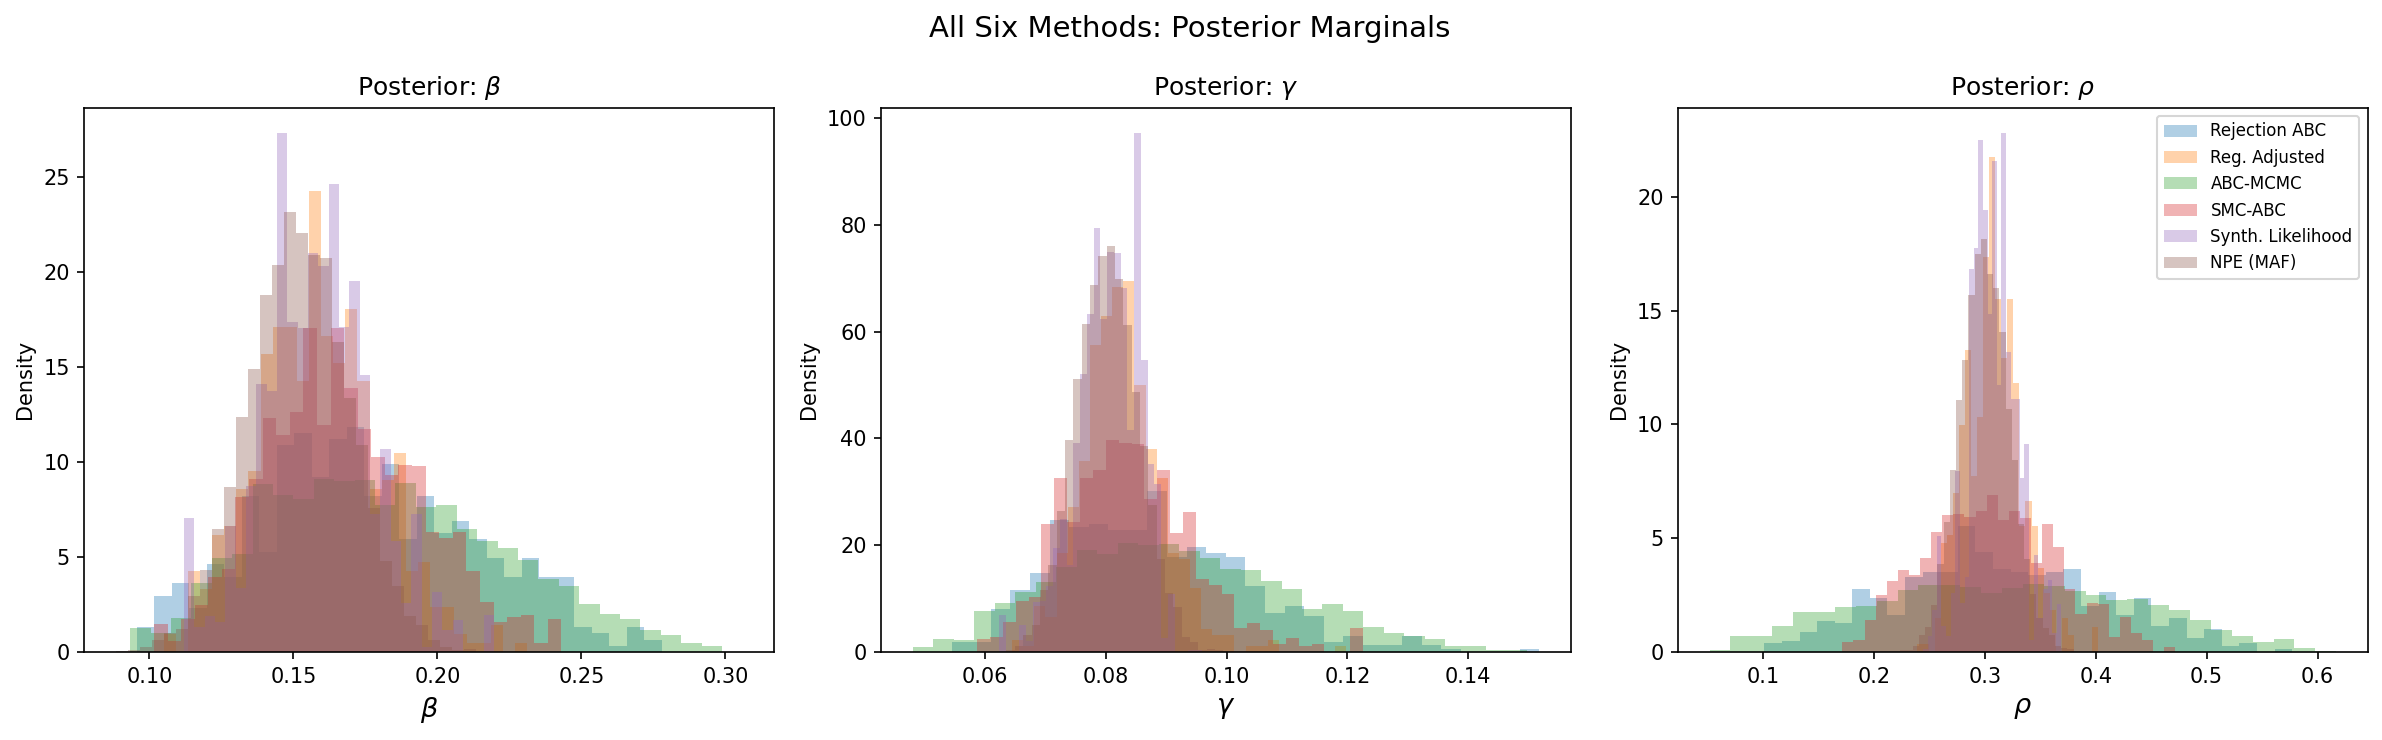
\includegraphics[width=0.80\textwidth]{../figures/all_methods_comparison.png}
\caption{Marginal posterior densities for $\beta$, $\gamma$, $\rho$ from all six methods. NPE (purple) and Synthetic Likelihood (purple) produce essentially overlapping, very tight posteriors; the classical ABC methods are progressively wider; ABC-MCMC is the widest, reflecting the inherent looseness imposed by its tolerance.}
\label{fig:all_methods}
\end{figure}

\paragraph{Discussion.}
\begin{itemize}[nosep, leftmargin=10pt]
\item \textbf{Point estimates agree closely across methods.} All six methods place $\beta$ in $[0.154, 0.182]$, $\gamma$ in $[0.080, 0.091]$ and $\rho$ in $[0.301, 0.316]$. This consistency is reassuring: it strongly suggests that the data and model are informative enough to constrain the parameters, and that the differences we see are about \emph{precision}, not \emph{bias}.
\item \textbf{NPE delivers the tightest posteriors at the lowest cost-per-precision.} It matches synthetic likelihood on $\rho$ (CI width $0.093$ vs.\ $0.098$) and slightly beats it on $\beta$, while running in $60\,$s versus $6{,}731\,$s --- a two-orders-of-magnitude speedup. Crucially, NPE reuses the very same $50{,}000$ simulations as the rejection ABC baseline, so its true cost over and above rejection ABC is the $\sim 17\,$s of training time.
\item \textbf{Synthetic likelihood is precise but expensive.} Each likelihood evaluation requires $N_r=200$ fresh simulations, so the $5{,}000$ MCMC iterations consume $10^6$ simulator calls. The acceptance rate is low ($7.4\%$), reflecting the difficulty of mixing in the tight high-likelihood region. The result is statistically excellent but computationally heavy.
\item \textbf{Regression adjustment is the best ``free'' upgrade.} It costs $0.013\,$s on top of rejection ABC, yet shrinks the $\rho$ CI from $0.39$ to $0.12$ --- a $3\times$ improvement. This is the cheapest single intervention in the report.
\item \textbf{SMC-ABC sits in the middle.} Its $\rho$ CI ($0.21$) is roughly half of rejection ABC's, but at the cost of a $4\times$ longer runtime. The progressive tolerance schedule worked smoothly (final $\varepsilon = 1.47$) and the effective sample size remained around $900$ throughout, so the method is well-tuned --- it is just inherently more expensive than the post-hoc regression adjustment.
\item \textbf{ABC-MCMC is the widest.} Its CIs are actually wider than rejection ABC's. With acceptance rate $34\%$ and ESS in the hundreds, the chain is mixing reasonably, but the tolerance ($\varepsilon = 3.01$) is slightly larger than the rejection ABC threshold to keep acceptance reasonable, and that looseness propagates into the posterior. ABC-MCMC is therefore not competitive on this problem; its main advantage --- targeted exploration of the posterior --- is undercut by the need to maintain a generous tolerance.
\end{itemize}

\paragraph{A note on amortisation.} NPE has a property that none of the other methods share: the trained network can be queried for \emph{any} new observed dataset in milliseconds, with no further simulation. If we received a second batch of $40$ replicates tomorrow under the same model, NPE would give us a posterior immediately while every other method would need to redo $\sim 10^4$--$10^6$ simulations. This makes NPE qualitatively different from the classical methods and especially attractive for applications where the same model is fitted repeatedly.

\section{Validation}

The preceding sections established that all six methods agree on point estimates and that NPE produces the tightest posteriors. Two questions remain: (i) are these posteriors \emph{calibrated} --- do they actually contain the true parameters at the claimed coverage level? --- and (ii) how much of NPE's apparent advantage is genuine statistical efficiency versus simply consuming a larger simulation budget?

\subsection{Synthetic-truth recovery}

To test calibration, we simulate $40$ synthetic replicates from a known ground truth $\theta^* = (\beta = 0.17,\; \gamma = 0.085,\; \rho = 0.30)$, chosen near the posterior medians from the real data. We then run the full inference pipeline --- rejection ABC ($50{,}000$ simulations, $q=1\%$) and NPE (MAF, same $50{,}000$ simulations) --- on this synthetic dataset and check whether the $95\%$ credible intervals cover $\theta^*$.

\begin{table}[htb]
\centering
\small
\begin{tabular}{lccccc}
\toprule
Parameter & True value & \multicolumn{2}{c}{Rejection ABC 95\% CI} & \multicolumn{2}{c}{NPE 95\% CI} \\
\cmidrule(lr){3-4} \cmidrule(lr){5-6}
 & & Interval & Covers? & Interval & Covers? \\
\midrule
$\beta$  & 0.170 & $[0.120,\; 0.269]$ & Yes & $[0.131,\; 0.211]$ & Yes \\
$\gamma$ & 0.085 & $[0.064,\; 0.124]$ & Yes & $[0.074,\; 0.097]$ & Yes \\
$\rho$   & 0.300 & $[0.136,\; 0.503]$ & Yes & $[0.258,\; 0.355]$ & Yes \\
\bottomrule
\end{tabular}
\caption{Synthetic-truth recovery. Both methods cover the true parameters within their 95\% credible intervals. NPE's intervals are $2$--$4\times$ narrower while still containing the truth.}
\label{tab:synthetic_truth}
\end{table}

\begin{figure}[htb]
\centering
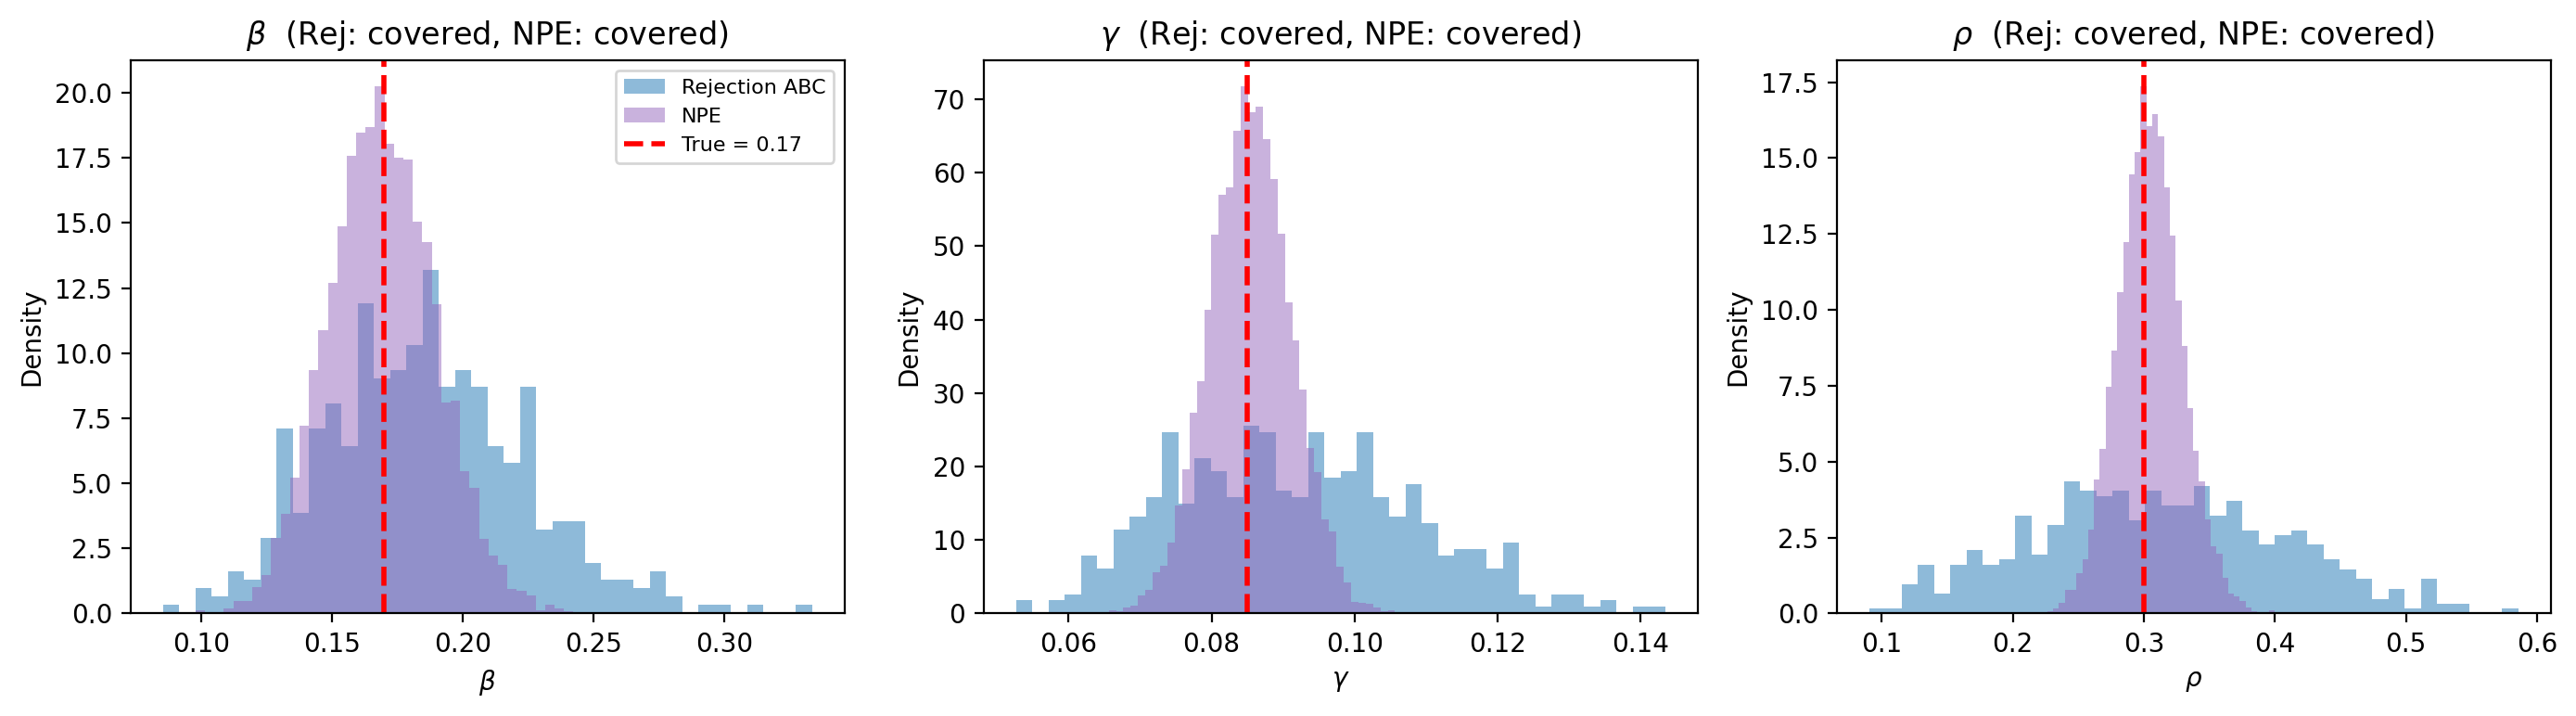
\includegraphics[width=0.85\textwidth]{../figures/synthetic_truth_recovery.png}
\caption{Posterior marginals from the synthetic-truth experiment. Dashed red lines mark the true parameter values. Both rejection ABC (blue) and NPE (purple) concentrate around the truth; NPE is substantially more precise.}
\label{fig:synthetic_truth}
\end{figure}

Table~\ref{tab:synthetic_truth} and Figure~\ref{fig:synthetic_truth} confirm that both methods recover the truth: all six intervals (three parameters $\times$ two methods) cover $\theta^*$. NPE's intervals are $2$--$4\times$ narrower than rejection ABC's while still containing the truth, indicating that the tighter NPE posteriors from the real-data analysis are not artefactually overconfident.

\subsection{Budget-matched comparison}

Table~\ref{tab:all_methods} shows that the six methods use very different simulation budgets (from $30{,}000$ to $10^6$). To disentangle statistical efficiency from sheer compute, we compare rejection ABC, SMC-ABC, and NPE each using approximately $50{,}000$ simulator calls. SMC-ABC is run with a budget cap and stops after the last complete generation within the budget (here, $7$ generations consuming ${\sim}50{,}000$ calls).

\begin{table}[htb]
\centering
\small
\begin{tabular}{lcccccc}
\toprule
Method & $\hat\beta$ & $\hat\gamma$ & $\hat\rho$ & $|\text{CI}_\beta|$ & $|\text{CI}_\gamma|$ & $|\text{CI}_\rho|$ \\
\midrule
Rejection ABC ($q=1\%$) & 0.173 & 0.087 & 0.308 & 0.140 & 0.060 & 0.352 \\
SMC-ABC (7 gen)         & 0.170 & 0.085 & 0.305 & 0.117 & 0.051 & 0.300 \\
NPE (MAF)               & 0.152 & 0.081 & 0.303 & 0.071 & 0.021 & 0.097 \\
\bottomrule
\end{tabular}
\caption{Budget-matched comparison at $50{,}000$ simulator calls. At equal budget, NPE achieves the tightest posteriors by a wide margin; SMC-ABC improves modestly on rejection ABC.}
\label{tab:budget_matched}
\end{table}

\begin{figure}[htb]
\centering
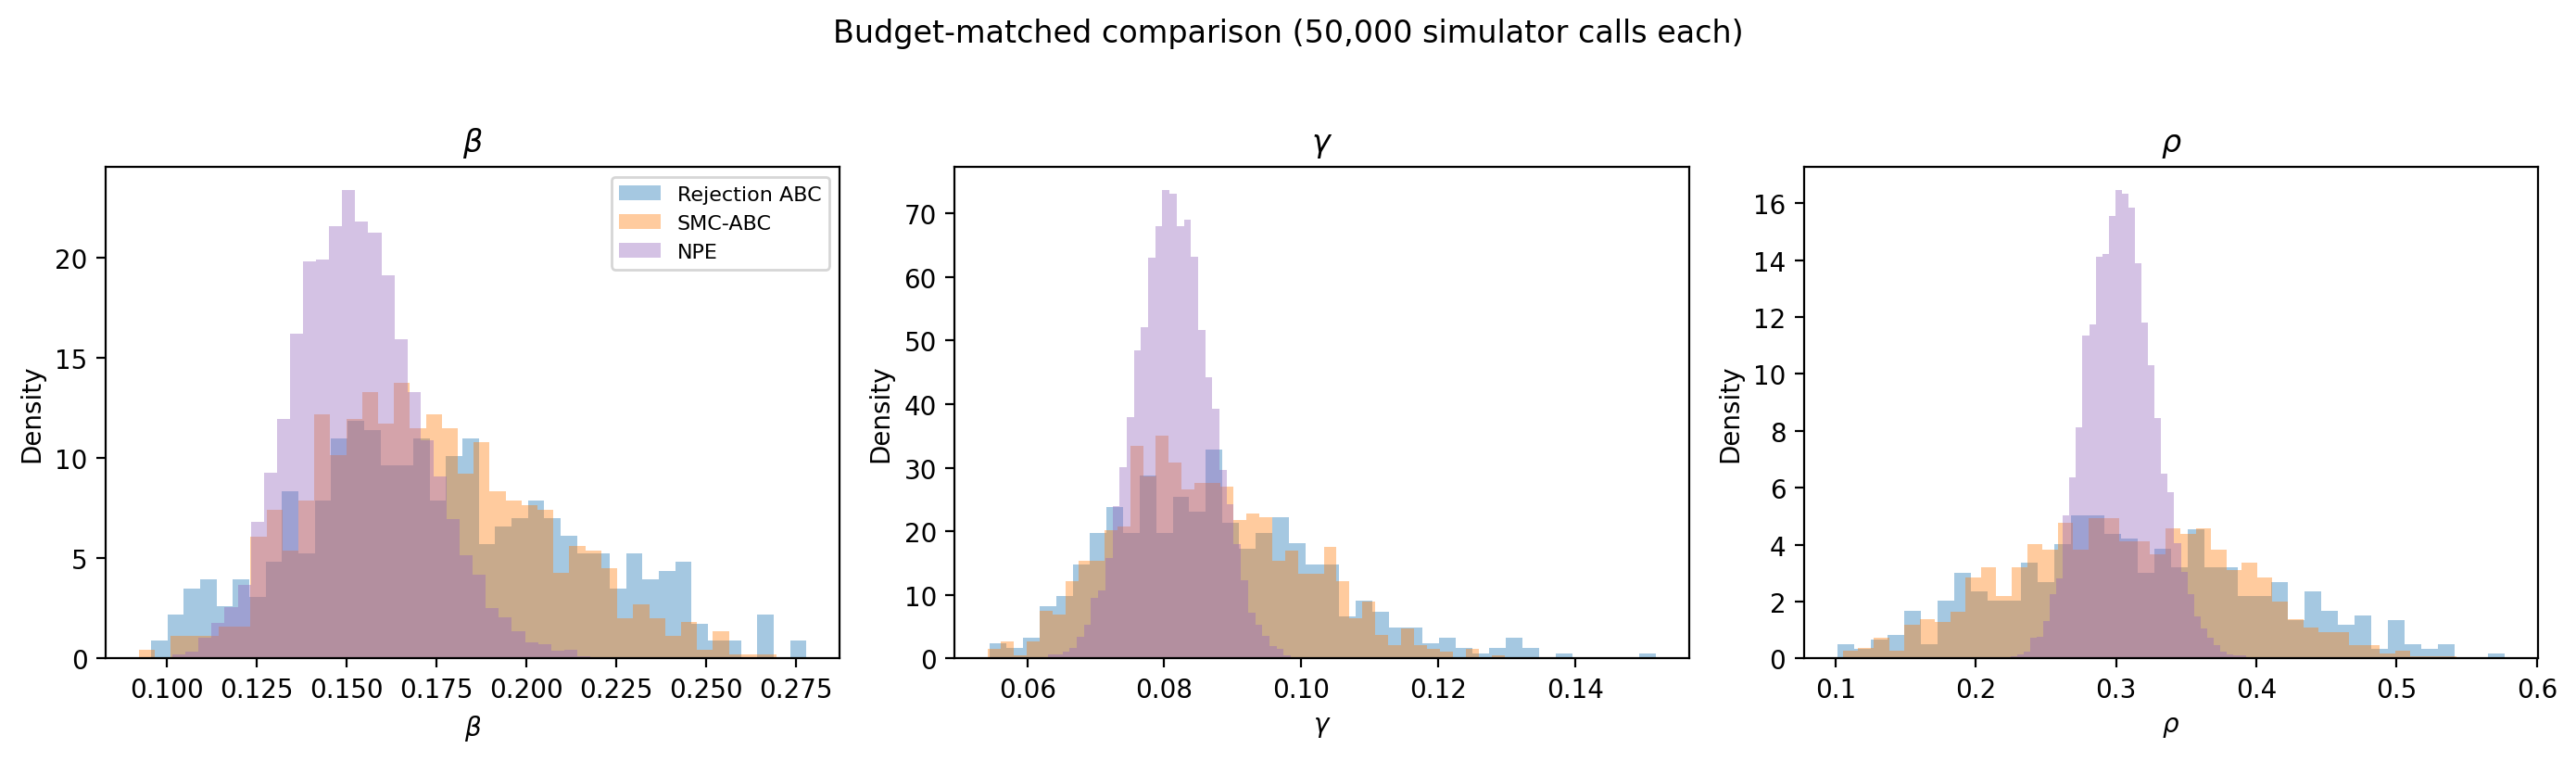
\includegraphics[width=0.85\textwidth]{../figures/budget_matched.png}
\caption{Marginal posteriors from the budget-matched comparison ($50{,}000$ simulator calls each). NPE (purple) is sharply concentrated; SMC-ABC (orange) is moderately tighter than rejection ABC (blue).}
\label{fig:budget_matched}
\end{figure}

At equal budget (Table~\ref{tab:budget_matched}, Figure~\ref{fig:budget_matched}), NPE's $\rho$ CI ($0.097$) is $3.6\times$ narrower than rejection ABC's ($0.352$) and $3.1\times$ narrower than SMC-ABC's ($0.300$). This confirms that NPE's advantage in Table~\ref{tab:all_methods} is genuine statistical efficiency --- it extracts more information per simulation --- rather than an artefact of consuming a larger budget.

\section{Conclusion}

We have applied six simulation-based inference methods to the problem of estimating $(\beta, \gamma, \rho)$ in an adaptive-network SIR epidemic model from $40$ observed replicates. The likelihood is intractable because the network co-evolves with the infection state, but the model is cheap to simulate, making SBI a natural framework. Our key findings are:

\begin{enumerate}[nosep, leftmargin=10pt]
\item \textbf{Summary statistics design dominates the inference.} The infected fraction time series alone leaves $\beta$ and $\rho$ strongly positively correlated ($\hat r = +0.886$) and the $\rho$ posterior almost as wide as the prior. Adding rewiring statistics reduces the $\rho$ CI width from $0.75$ to $0.40$, and combining all $12$ summaries gives the best overall results.
\item \textbf{Neural Posterior Estimation is the most efficient method.} Reusing the same $50{,}000$ simulations as the rejection ABC baseline, NPE produces the tightest credible intervals among all six methods (e.g.\ $|\text{CI}_\rho| = 0.093$) in $60\,$seconds total. It also offers cheap amortised inference for future datasets.
\item \textbf{Regression adjustment is a remarkable free lunch.} A few lines of weighted least squares on top of rejection ABC reduces the $\rho$ CI by a factor of three at essentially zero cost.
\item \textbf{Synthetic likelihood matches NPE in precision but is $112\times$ slower.} It would be the method of choice if we did not trust a neural network on this problem, or if the simulation budget were too small to train one.
\item \textbf{ABC-MCMC is not competitive on this problem.} The need to keep the tolerance loose enough for the chain to mix produces a posterior wider than that of plain rejection ABC.
\end{enumerate}

\noindent In aggregate, the methods agree on the underlying parameter values, and the spread of methods provides cross-validation: the inference is reliable. For practical work on this kind of model we would recommend starting with rejection ABC (for quick prototyping and MAD calibration), then applying regression adjustment (free precision boost), and finally training NPE on the same simulations for the most accurate and amortised result.

\bibliographystyle{plainnat}
\bibliography{references}

\end{document}
